\documentclass{article}
\usepackage[margin=0.5in]{geometry}
\usepackage{graphicx}
\usepackage{verbatim}
\usepackage{hyperref}
\title{Safety: Start at the  Bottom and Stay There!} 
\author{Evan Trevathan}
\date{}
\begin{document}
\pagenumbering{gobble}
\maketitle 
\section*{Goal} 
Predict likelihood of the next safety incident being a recordable incident using "Heinrich's Accident Pyramid" theory.
\begin{center}
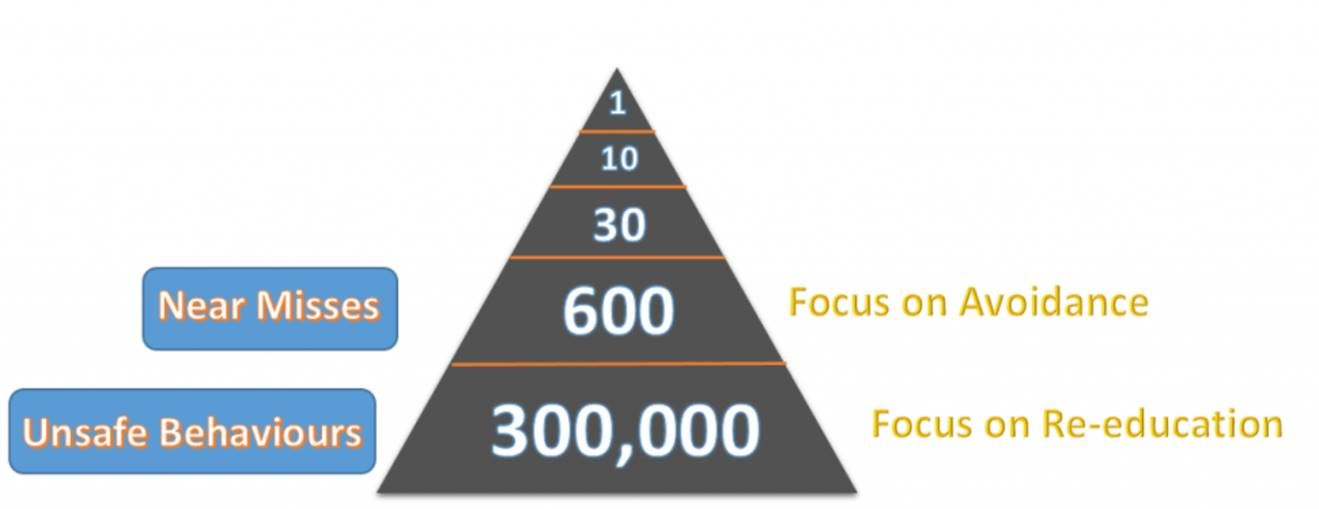
\includegraphics[scale=.65]{SafetyTriangle.jpg}
\end{center}
\section*{Data} 
\begin{enumerate}
	\item The dataset considered was the SafetyApp data:
	\begin{itemize}
		\item Excluded all records that were soft deleted.
		\item Pulled data on 4/18/2018
		\item 10,698 rows
		\item 88 original features
		\item Utilized 13 features from original dataset plus 1 feature from Asset table.
		\item Created/Altered 4 features
		\item All data manipulation performed in SQL
	\end{itemize}
	\item Could utilize the SafetyPlus data if necessary:
	\begin{itemize}
		\item Would need to map to selected feature set.
		\item 28,506 rows
		\item 562 original features
	\end{itemize}
\end{enumerate}

\section*{Approach} 
Implement Multinomial Time Series Regression to model the likelihood the next data entry point is a recordable incident. We will classify the data as either recordable or non-recordable and utilize the ratios from Heinrich's Accident Pyramid theory applied to BP Lower 48 Safety entries.

\begin{comment}
https://www.hlp.rochester.edu/resources/WOMM/BarrFrank.pdf
\end{comment}
\section*{Project Progression} 
\begin{enumerate}
	\item Feature selection and creation done.
	\item Dataset loaded into Pandas.
	\item Research has begun on algorithm details.
\end{enumerate}
\begin{comment}
\section*{Model Pipeline Code} 
TBD    
\end{comment}
\end{document}
